\section{Clase 20}
Curva de coexistencia (isoterma en el diagrama $PV$)

\begin{figure}[h!]
	\centering
	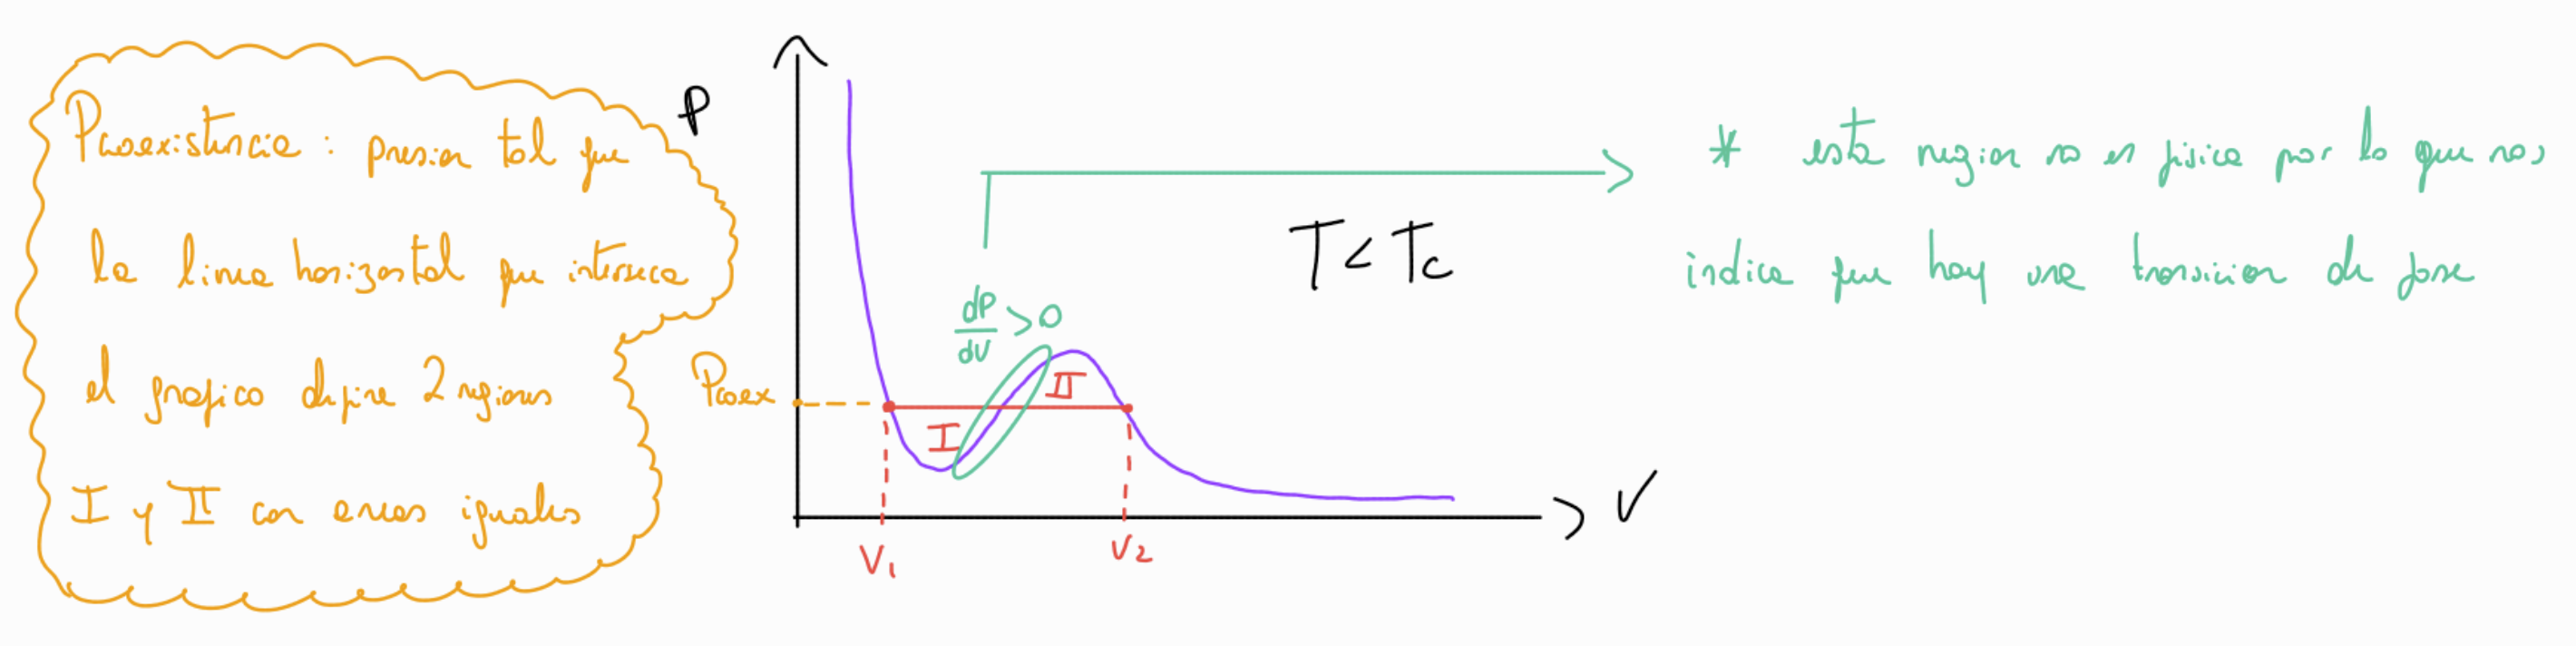
\includegraphics[scale=0.3]{fig/20-1.png}
\end{figure}
Construcción de Maxwell: Áreas de las regiones $I$ y $II$ son iguales (en el diagrama $PV$)
\begin{itemize}
	\item Para $V<V_1$, el fluido está en fase líquida\\
	\item Para $V>V_2$, el fluido está en fase gaseosa\\
	\item Para $V_1<V<V_2$, coexistencia entre ambas fases (líquida y gaseosa)
\end{itemize}
A $T$ constante, la compresión del fluido ocurre entre $V_2$ y $V_1$ ocurre a $P$ constante.

Existe un \textit{calor latente de transición}


\begin{ej}
	Sea $L$ el calor latente de transición del fluido. Calculo el volúmen de gas convertido a líquido si la transición a $P$ y $T$ constante, es la fase de coexistencia y si $M$ partículas sufren la transición de fase.
	
	\underline{Hint:} La energía necesaria para que $M$ partículas sufran la transición de fase es
	\begin{equation}
  E=LM
\end{equation}
donde $L$ es la energía por partícula.
\end{ej}

\begin{sol}
Usamos $F$ porque es un proceso a $T$, $P$ y $N$ constante,
	\begin{align}
  \dd E&=T\dd S-P\dd V+\m \dd N\\
  F&=E-TS
\end{align}
Recordemos que en fase de coexistencia como queremos mantener $P$ constante el proceso, que ocurre hay una transición de fase,
\begin{align}
  \dd F&=-S\cancel{\dd T }-P\dd V+\m \cancel{\dd N}\\
  \dd F&=-P\dd V\\
  \Delta F&=-P\Delta V
\end{align}
donde $-P\Delta V$ es el trabajo necesario para cambiar de fase. Usando la definición de calor latente
\begin{align}
  \Delta F&=-P\Delta V=LM
\end{align}
entonces nos queda que
\begin{equation}
  \Delta V=-\frac{LM}{P}
\end{equation}
Notar que $\Delta V<0$.

Al comprimir el gas, parte de este se transforma en líquido (a $P$ y $T$ constante). El volúmen de gas contenido es líquido puede aproximarse como
\begin{equation}
  V_{\text{gas $\to$ líquido}}=-\Delta V
\end{equation}
considerando que
\begin{equation}
  V_{\text{líquido}}\ll V_{\rm gas}
\end{equation}
luego, $V_{\text{gas $\to$ líquido}}$ será aproximadamente
\begin{equation}
\boxed{  V_{\text{gas $\to$ líquido}}=\frac{LM}{P}}
\end{equation}
\end{sol}

\subsection{Derivación de la construcción de Maxwell}
En la fase de coexistencia, de la Clase \ref{clase:2}
\begin{equation}
  P_{\rm gas}=P_{\text{líquido}},\qquad  T_{\rm gas}=T_{\text{líquido}},\qquad  \m _{\rm gas}=\m _{\text{líquido}}
\end{equation}
por otro lado, de la relación de Euler
\begin{equation}
  E=Ts-PV+\m N
\end{equation}
y de la primera ley
\begin{equation}
  \dd E=T\dd S-P\dd V+\m \dd N
\end{equation}
Usando ambas
\begin{equation}
  N\dd\m =-S\dd T+V\dd P
\end{equation}
En la curva isoterma ($T$ constante), $\dd T=0\rightarrow N\dd\m =V\dd P$. Integrando a ambos lados, nos queda
\begin{align}
  \m_{\rm gas}-\m_{\text{líquido}}&=\int_{\text{líquido}}^{\rm gas}\left(\frac{V}{N}\right)\dd P\\
  &=\eval{P_v}_{\text{liq}}^{\rm gas}-\int_{\rm liq}^{\rm gas}P\dd v,\qquad v=\frac{V}{N}
\end{align}
Entonces
\begin{equation}
  \m_{\rm gas}-\m_{\text{líquido}}=P_{\rm gas}v_{\rm gas}-P_{\rm liq}v_{\rm liq}-\int_{\rm liq}^{\rm gas}P\dd v
\end{equation}
pero recordemos que
\begin{equation}
  \m_{\rm liq}=\m_{\rm gas}\qquad P_{\rm liq}=P_{\rm gas}=P_{\rm coexistencia}
\end{equation}
nos queda
\begin{equation}
  0=P_{\rm coex}(v_{\rm gas}-v_{\rm liq})-\int_{\rm liq}^{\rm gas}P\dd v
\end{equation}
Podemos hacer un cambio de variable, usando que $\dd v=\dd V/N$
\begin{equation}\label{20.star}
  0=\frac{P_{\rm coex}}{N}(V_{\rm gas}-V_{\rm liq})-\frac{1}{N}\int_{V\rm liq}^{V\rm gas}P(V)\dd V\qquad  (\star)
\end{equation}
en donde $P(V)$ a $T$ constante está dado por la ecuación de estado de Van der Walls.

La condición \eqref{20.star} puede interpretarse geométricamente como que $P_{\rm coex}$ es aquel valor de $P$ tal que \textit{las regiones $I$ y $II$ del diagrama anterior tiene igual área.}

\begin{figure}[h!]
	\centering
	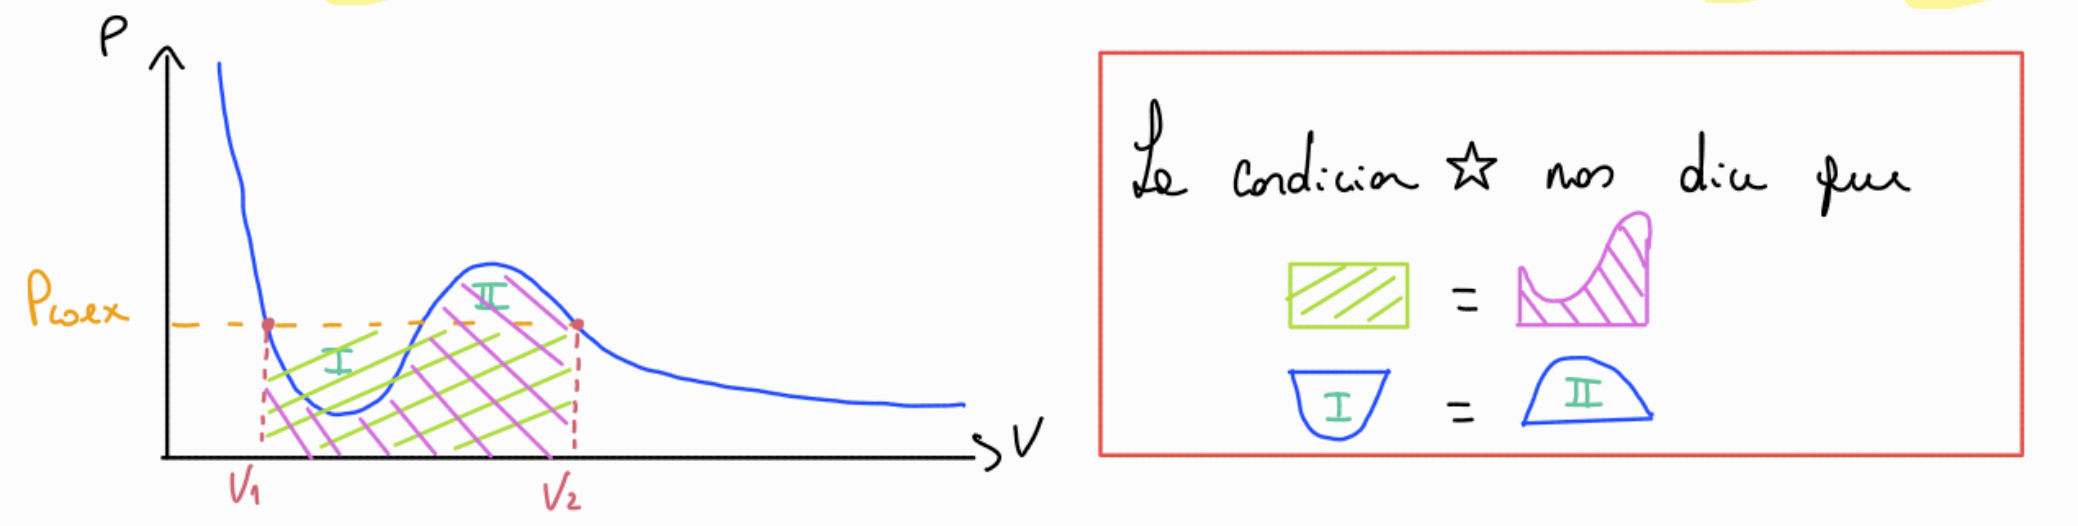
\includegraphics[scale=0.4]{fig/20-star.png}
\end{figure}

Así, encontramos los siguientes puntos críticos $T_c$, $P_c$ y $V_c$ donde ocurre la transición de fase. Usaremos las siguientes variables:
\begin{equation}
  p=\frac{P}{a\r_s^2},\qquad t=\frac{\k T}{a\r_s	},\qquad v=\r_s\frac{V}{N}=\frac{\r_s}{\r }
\end{equation}
tal que $\r$, $t$ y $v$ son adimensionales.

Entonces, la ecuación de estado se escribe:
\begin{equation}
\boxed{  P=\frac{t}{v-1}-\frac{1}{v^2}}
\end{equation}

Para $T<T_c$ hay dos puntos donde $(\pdv*{P}{V})|_{T,N}=0$ es uno de tales puntos
\begin{equation}
\eval{  \pdv[2]{P}{V}}_{T,N}<0
\end{equation}
sin embargo es el \textit{punto crítico},
\begin{equation}\label{20.2star}
\boxed{  \eval{\pdv{P}{v}}_{t}=\eval{\pdv[2]{V}{v}}_t=0}
\end{equation}
Si la segunda derivada no fuera cero, $p(v)$ no sería monótona. De \eqref{20.2star} resulta en las siguientes condiciones
\begin{equation}
  \frac{t_c}{(v_c-1)^2}=\frac{2}{v_c^2}
\end{equation}
y
\begin{equation}
  \frac{2t_c}{(v_c-1)^3}=\frac{6}{v_c^4}
\end{equation}
Finalmente, considerando la ecuación de estado de Van der Walls misma
\begin{equation}
  p_c=\frac{t_c}{v_c-1}-\frac{1}{v_c^2}
\end{equation}
Resolviendo el sistema, obtenemos
\begin{equation}
  v_c=3,\qquad t_c=\frac{8}{27},\qquad p_c=\frac{1}{27}
\end{equation}
Finalmente en términos de variables físicas, tenemos
\begin{equation}
  \r_c=\left(\frac{N}{V}\right)_c=\frac{\r_s}{3},\qquad T_c=\frac{8}{27}a\r_s,\qquad P_c=\frac{1}{27}a\r_s^2
\end{equation}
Estos corresponden a los parámetros termodinámicos del punto crítico de la ecuación de Van der Waals.

\subsection{Ecuación de Clausius-Clapeyron}
A lo largo de la curva de coexistencia $P$ vs $T$ se cumple
\begin{equation}
	\boxed{\dv{P}{T}=\frac{L/T}{(V/N)_{\rm gas}-(V/N)_{\rm liq}}}
\end{equation}

Considere una curva de coexistencia $P$ vs $T$
\begin{figure}[h!]
	\centering
	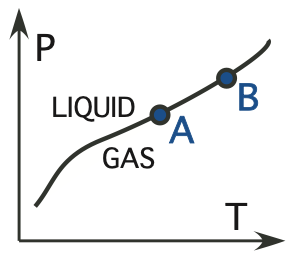
\includegraphics[scale=0.4]{fig/CP-eq.png}
\end{figure}

La curva demarca la transición entre las fases líquido y gaseosa. A lo largo de la curva se tiene:
\begin{align}
  \m_{\rm liq}&=\m_{\rm gas}\\
  \m_{\rm liq}^{(B)}-\m_{\rm liq}^{(A)}&=\m_{\rm gas}^{(B)}-\m_{\rm gas}^{(A)}
\end{align}
y como $N\dd\m=-S\d T+V\dd P$, se tiene
\begin{equation}
  -\left(\frac{S}{N}\right)_{\rm liq}\dd T+\left(\frac{V}{N}\right)_{\rm liq}\dd P= -\left(\frac{S}{N}\right)_{\rm gas}\dd T+\left(\frac{V}{N}\right)_{\rm gas}\dd P
\end{equation}
\begin{equation}
  \implies \dv{P}{T}=\frac{\left(\frac{S}{N}\right)_{\rm gas}-\left(\frac{S}{N}\right)_{\rm liq}}{\left(\frac{V}{N}\right)_{\rm gas}-\left(\frac{V}{N}\right)_{\rm liq}}
\end{equation}
Ahora, como
\begin{equation}
  L=\frac{T\Delta S}{N}
\end{equation}
siendo $L$ el calor latente de cambio de fase, ya sea a $P$ o $V$ constante, se tiene
\begin{equation}
  \left(\frac{S}{N}\right)_{\rm gas}-\left(\frac{S}{N}\right)_{\rm liq}=\frac{L}{T}
\end{equation}
y por tanto
\begin{equation}
	\boxed{\dv{P}{T}=\frac{L/T}{(V/N)_{\rm gas}-(V/N)_{\rm liq}}}
\end{equation}








































































